\documentclass[12pt, a4paper]{article}
\usepackage{graphicx}
\graphicspath{ {./imgs/} }
\usepackage{float}
\usepackage{listings}
\usepackage{color}

\definecolor{codegreen}{rgb}{0,0.6,0}
\definecolor{codegray}{rgb}{0.5,0.5,0.5}
\definecolor{codeorange}{rgb}{1,0.49,0}
\definecolor{backcolour}{rgb}{0.95,0.95,0.96}

\lstset{
  backgroundcolor=\color{backcolour},   
  commentstyle=\color{codegray},
  keywordstyle=\color{codeorange},
  numberstyle=\tiny\color{codegray},
  stringstyle=\color{codegreen},
  basicstyle=\ttfamily\footnotesize,
  breakatwhitespace=false,         
  breaklines=true,                 
  captionpos=b,                    
  keepspaces=true,                 
  numbers=left,                    
  numbersep=5pt,                  
  showspaces=false,                
  showstringspaces=false,
  showtabs=false,                  
  tabsize=2,
  xleftmargin=10pt,
}
\renewcommand{\lstlistingname}{Code}

\counterwithin{figure}{section}

% javascript definition

\definecolor{lightgray}{rgb}{.9,.9,.9}
\definecolor{darkgray}{rgb}{.4,.4,.4}
\definecolor{purple}{rgb}{0.65, 0.12, 0.82}

\lstdefinelanguage{javascript}{
  keywords={typeof, new, true, false, catch, function, return, null, catch, switch, var, if, in, while, do, else, case, break, let, const, type},
  keywordstyle=\color{blue}\bfseries,
  ndkeywords={class, export, boolean, throw, implements, import, this},
  ndkeywordstyle=\color{darkgray}\bfseries,
  identifierstyle=\color{black},
  sensitive=false,
  comment=[l]{//},
  morecomment=[s][\color{purple}]{/*}{*/},
  %morecomment=[s][\color{codegreen}]{:}{=},
  %morecomment=[s][\color{codegreen}]{:}{;},
  commentstyle=\color{purple}\ttfamily,
  stringstyle=\color{red}\ttfamily,
  morestring=[b]',
  morestring=[b]"
}

\lstset{
  language=JavaScript,
  backgroundcolor=\color{lightgray},
  extendedchars=true,
  basicstyle=\footnotesize\ttfamily,
  showstringspaces=false,
  showspaces=false,
  numbers=left,
  numberstyle=\footnotesize,
  numbersep=9pt,
  tabsize=2,
  breaklines=true,
  showtabs=false,
  captionpos=b
}

%to write code:
%\begin{lstlisting}[language=java, caption={my caption}]
%    
%\end{lstlisting}

%to insert an image
%\begin{figure}[H]
%  \centering
%  \includegraphics[width=\columnwidth]{img.png}
%  \caption{description of the image}
%\end{figure}

\title{Web Architectures - Delivery 3}
\author{Marrocco Simone}

\begin{document}
  \maketitle
  \begin{figure}[H]
    \centering
    
\includegraphics[scale=0.35]{unitn.png}
  \end{figure}
  \tableofcontents
  \pagebreak

  \section{Introduction}
  In this assignment we were asked to create a simple spreadsheet webapp. In particular, we needed to code the connection between users and the server. The source code for computing the cell values given a formula was given.

  For the front end, the javascript code was written in typescript and then compiled, since it offers many benefits like type definition, bug detection and it can compile to ES2016 standard while being written with all the modern javascript features. It is given both the typescript and the compiled javascript file, however the latter is not much readable and should not be modified, since its purpose is just to be served. The ts config file is also given, and it is the standard one.

  \section{Single Page application}
  For the first task, the client needs to send an http request for a cell formula modification: the server would then respond with the modifications to show.

  \subsection{Front End Javascript}
  \subsubsection{HTML variables}
  \begin{lstlisting}[language=javascript, caption={globals}]
    //@ts-ignore
    const n_rows: number = n_rows;

    // get html references
    const d = document;
    const input = <HTMLInputElement>d.getElementById("modify-cell");
    const label = <HTMLLabelElement>d.getElementById("modify-cell-label");
    const submit_button = <HTMLButtonElement>d.getElementById("modify-cell-submit");
    if (!(input && label && submit_button))
      throw new Error(
        "Html file not correct format or you didn't import with 'defer'"
      );
  \end{lstlisting}
  
  We start the file with the references to the elements that makes the form used to send the formula updates to the server. This is made possible by the tag \textit{defer} in the script tag, which loads the javascript only after the html is rendered.

  In the first line, we use a trick to read in the javascript file the \textit{n\_rows} variable set up in the jsp. This is not required to make the file work, but it makes writing the file much easier since the variable is referenced.

  \subsubsection{Types}
  \begin{lstlisting}[language=javascript, caption={types}]
    /** request body to use to the server when informing of changes */
    type Update = {
      cell: string;
      formula: string;
    };

    /** json of the changes to do from the server */
    type ServerChanges = {
      changes: [
        {
          cell: string;
          value: string;
          formula: string;
        }
      ];
    };

    /** json of error from the server */
    type ServerPostError = {
      reason: string;
    };

    /** type of the data structure used to save the data about the cells */
    type CellValueMap = {
      [cell_id: string]: {
        formula: string;
        shown_value: string;
      };
    };
  \end{lstlisting}

  One of the main advantages of typescript is that we can have a clear idea about the objects we are using by defining their type definition. We can also use them to determine what the response object will be.

  \pagebreak

  \subsubsection{Initialization}
  \begin{lstlisting}[language=javascript, caption={initialization}]
    /** data structure to save the data about the cells */
    const cell_value_map: CellValueMap = {};
    initCellValueMap();

    /** initialize the cell_value_map by asking the server */
    function initCellValueMap() {
      for (let i = 0; i < n_rows; i++)
        for (let j = 1; j <= n_rows; j++) {
          const letter = String.fromCharCode("A".charCodeAt(0) + i);
          cell_value_map[letter + j] = {
            formula: "",
            shown_value: "",
          };
        }

      getStartingValues();
    }

    /** get the starting values from the server */
    async function getStartingValues() {
      try {
        const res_json = await fetch(url, {
          method: "GET",
        });
        const res: ServerChanges & ServerPostError = await res_json.json();

        if (res.changes) {
          modifyCells(<ServerChanges>res);
        } else {
          alert(`Server returned error: ${res.reason}`);
        }
      } catch (e: any) {
        console.error(e);
        // alert(`Something went wrong!\nError receiving changes: ${e.message}`);
      }
    }
  \end{lstlisting}

  We initialize the file by creating the data structure \textit{cell\_value\_map}, which will contains the informations about our cells, which all start with default values. Then we do a GET request to the server, asking if there are cell already written. This means the spreadsheet remains the same even if we refresh the page, since the data is also stored on the server.

  \subsubsection{Selecting a cell}
  \begin{lstlisting}[language=javascript, caption={To select a cell}]
    /**
    * function called from a cell onclick event.
    * It changes the current_cell, by coloring it red and
    * enables input modification.
    */
    function clickedCell(cell_id: string) {
      const previous_cell_id = current_cell_id;
      resetClick();
      
      if (cell_id === previous_cell_id) return;
      
      const current_cell = document.getElementById(cell_id);
      if (!current_cell) return;
      current_cell.style.outline = "5px solid green";
      const formula = cell_value_map[cell_id].formula;
      current_cell.textContent = formula;
      input.value = formula;
      
      current_cell_id = cell_id;
      enableModify(cell_id);
      }
      
    /**
    * function called when the cell is not clicked anymore,
    * either because a new one is clicked or the cell is double clicked.
    * If the formula changed, send the server a change cell request
    */
    function resetClick() {
      const formula = input.value;
      input.value = "";
      input.disabled = true;
      label.textContent = "Select a cell to modify it";
      submit_button.disabled = true;
    
      const previous_cell = document.getElementById(current_cell_id);
      if (previous_cell) {
        previous_cell.style.outline = "0px solid black";
        previous_cell.textContent = cell_value_map[current_cell_id].shown_value;
        if (formula !== cell_value_map[current_cell_id].formula)
          serverParseFormula(formula);
      }
      current_cell_id = "";
    }
    
    /** enable the form input and button to modify the cell value */
    function enableModify(cell_id: string) {
      input.disabled = false;
      input.name = `new_${cell_id}_value`;
      input.focus();
      label.textContent = `Selected cell: ${cell_id}`;
      submit_button.disabled = false;
    }
    
    /** when something is typed in the input, changes the cell text to keep up */
    function inputChanged() {
      const current_cell = document.getElementById(current_cell_id);
      if (current_cell) {
        current_cell.textContent = input.value;
      }
    }

    /**
    * when the input form is submitted, send data to the server.
    * It prevents default behaviour
    */
    function submitInput(event: SubmitEvent) {
      event.preventDefault();

      const current_cell = document.getElementById(current_cell_id);
      if (current_cell) {
        resetClick();
      }
    }
  \end{lstlisting}

  When a cell is clicked, the function \textit{clickedCell} is called and we give the focus to the form, enable the modification of the form (with \textit{enableModify}), highlight the cell and change its text from the cell value to the cell formula. Changes to the input are reflected to the cell with the function \textit{inputChanged}.

  If there was already a selected cell, we first reset the click with \textit{resetClick} by resetting the form and the cell, and if the formula was changed the new one is sent to the server with \textit{serverParseFormula}.

  Of course, the user could send the new formula by just confirming the form, which calls \textit{submitInput}. In this case, we do not want to use the default behaviour of the form tag, but simply call \textit{resetClick} like before.

  \subsubsection{Sending changes to the server}
  \begin{lstlisting}[language=javascript, caption={Send changes}]
    /** inform the server of a cell modification, then use modifyCells() */
    async function serverParseFormula(formula: string) {
      if (formula.includes('"')) return alert('Invalid " character inside input');
      const server_req: Update = {
        cell: current_cell_id,
        formula,
      };

      try {
        const res_json = await fetch(url, {
          method: "POST",
          body: JSON.stringify(server_req),
        });
        const res: ServerChanges & ServerPostError = await res_json.json();

        if (res.changes) {
          modifyCells(<ServerChanges>res);
        } else {
          console.log(`POST request ERROR: ${res.reason}`);
          alert(`You made an invalid request\nReason: ${res.reason}`);
        }
      } catch (e: any) {
        console.error(e);
        alert(`Something went wrong!\nError sending changes: ${e.message}`);
      }
    }

    /** modify the cells as said from the server */
    async function modifyCells(res: ServerChanges) {
      if (!res.changes.length) return;

      console.table(res.changes);
      for (const c of res.changes) {
        const { cell: cell_id, value, formula } = c;

        const cell = document.getElementById(cell_id);
        if (!cell) continue;

        /** if the formula is empty, we want to show the cell as empty */
        const new_value = formula ? value : "";
        cell.textContent = new_value;
        cell_value_map[cell_id].shown_value = new_value;
        cell_value_map[cell_id].formula = formula;
      }
    }
  \end{lstlisting}

  The function \textit{serverParseFormula} is used to send a new formula to the server via POST method and receive the changes, by creating the correct JSON. 

  The changes are then shown with \textit{modifyCells}, which was also previously used by the GET method, since both method return the same JSON structure.

  \subsection{Back End Java}
  A single class was created, \textit{Server.java}, which is used as a Servlet that deliver both GET and POST methods and uses the \textit{SSEngine} given to execute the cell calculations, initialized in the \textit{init} method.

  \subsubsection{GET Method}
  \begin{lstlisting}[language=java, caption={GET route}]
    public void sendMessage(HttpServletResponse res, String msg, String contentType) throws IOException {
        res.setContentType(contentType);

        res.setHeader("Access-Control-Allow-Origin", "*");
        res.setHeader("Connection", "Keep-Alive");
        res.setHeader("Cache-Control", "no-cache");
        res.setCharacterEncoding("UTF-8");
        res.getWriter().write(msg);
        res.getWriter().flush();
    }
    
    public void sendUpdate(HttpServletResponse res, Set<Cell> modified_cells) throws IOException {
        String msg = modifiedCellsToString(modified_cells);
        sendMessage(res, msg, "text/application-json");
    }
    
    @Override
    public void doGet(HttpServletRequest req, HttpServletResponse res) throws IOException {
        System.out.println("\nNew user accessing");
        Set<Cell> modified_cells = engine.getUsedCells();
        sendUpdate(res, modified_cells);
    }
  \end{lstlisting}

  The GET method simply returns the current cells. The \textit{modifiedCellsToString} method converts the current cells to a JSON and filter the empty ones.

  Methods to send an update were created since both the GET and the POST routes use them.

  \subsubsection{POST Method}
  \begin{lstlisting}[language=java, caption={POST route}]
    public void sendErrorResponse(HttpServletResponse res, String reason) throws IOException {
        String msg = "{\"reason\": \"" + reason + "\"}";
        res.setStatus(400);
        sendMessage(res, msg, "text/application-json");
    }

    @Override
    public void doPost(HttpServletRequest req, HttpServletResponse res) throws IOException {
        System.out.println("\nNew update: ");

        String json_string = req.getReader().lines().collect(Collectors.joining(System.lineSeparator()));
        Pattern p = Pattern.compile("\\{\"cell\":\"(\\S+)\",\"formula\":\"(\\S*)\"}");
        Matcher m = p.matcher(json_string);

        if (!m.find()) {
            System.out.println("Incorrect JSON format. Regex not correct");
            sendErrorResponse(res, "Incorrect JSON format");
            return;
        }

        String cell = m.group(1);
        String formula = m.group(2);

        if (cell.contains("\"") || formula.contains("\"")) {
            System.out.println("Incorrect JSON format. It contains other fields as well");
            sendErrorResponse(res, "Incorrect JSON format. add only a cell and a formula field");
            return;
        }

        System.out.println("cell: "+cell+", formula: "+formula);
        Set<Cell> modified_cells = engine.modifyCell(cell, formula);
        if (modified_cells == null) {
            System.out.println("Circular Dependencies");
            sendErrorResponse(res, "Circular Dependencies");
            return;
        }

        sendUpdate(res, modified_cells);
        System.out.println();
    }    
  \end{lstlisting}
  The POST method parses the JSON. In case of errors, uses the \textit{sendErrorResponse} method to inform of the bad request, along with the 400 status. Otherwise, uses the engine method \textit{modifyCell} to execute the new formula and return the modified cells.

  \subsection{Results}
  \begin{figure}[H]
    \centering
    \begin{minipage}{.5\textwidth}
      \centering
      
\includegraphics[scale=0.3]{spreadsheet-empty.png}
      \caption{Blank Canvas}
    \end{minipage}%
    \begin{minipage}{.5\textwidth}
      \centering
      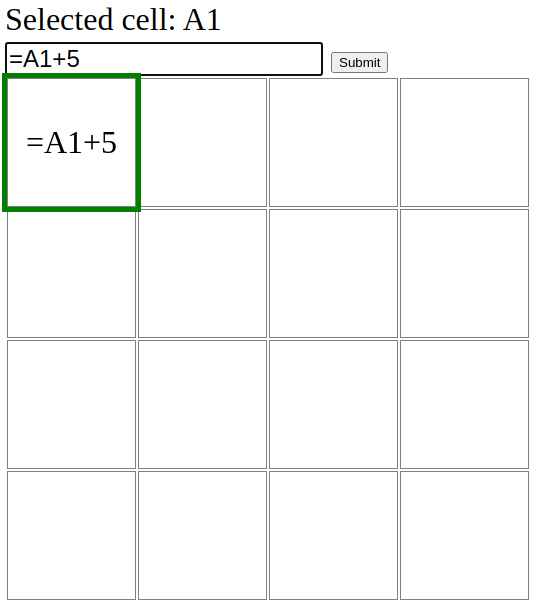
\includegraphics[scale=0.3]{spreadsheet-selected.png}
      \caption{Cell selected}
    \end{minipage}
  \end{figure}
  \begin{figure}[H]
    \centering
    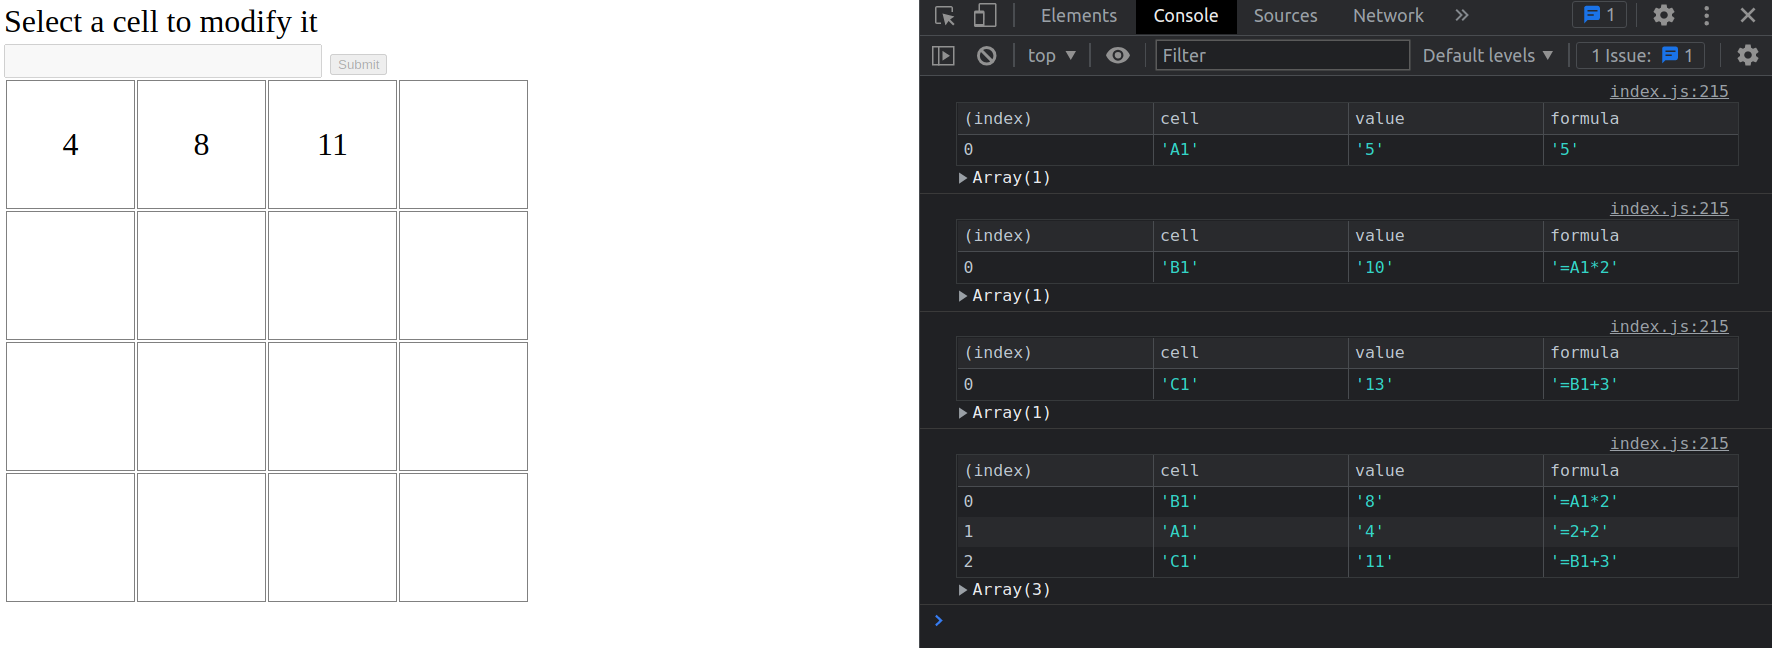
\includegraphics[width=\columnwidth]{spreadsheet-POST.png}
    \caption{Sending new formulas to the server. We can see how we receive back the changes}
  \end{figure}
  \begin{figure}[H]
    \centering
    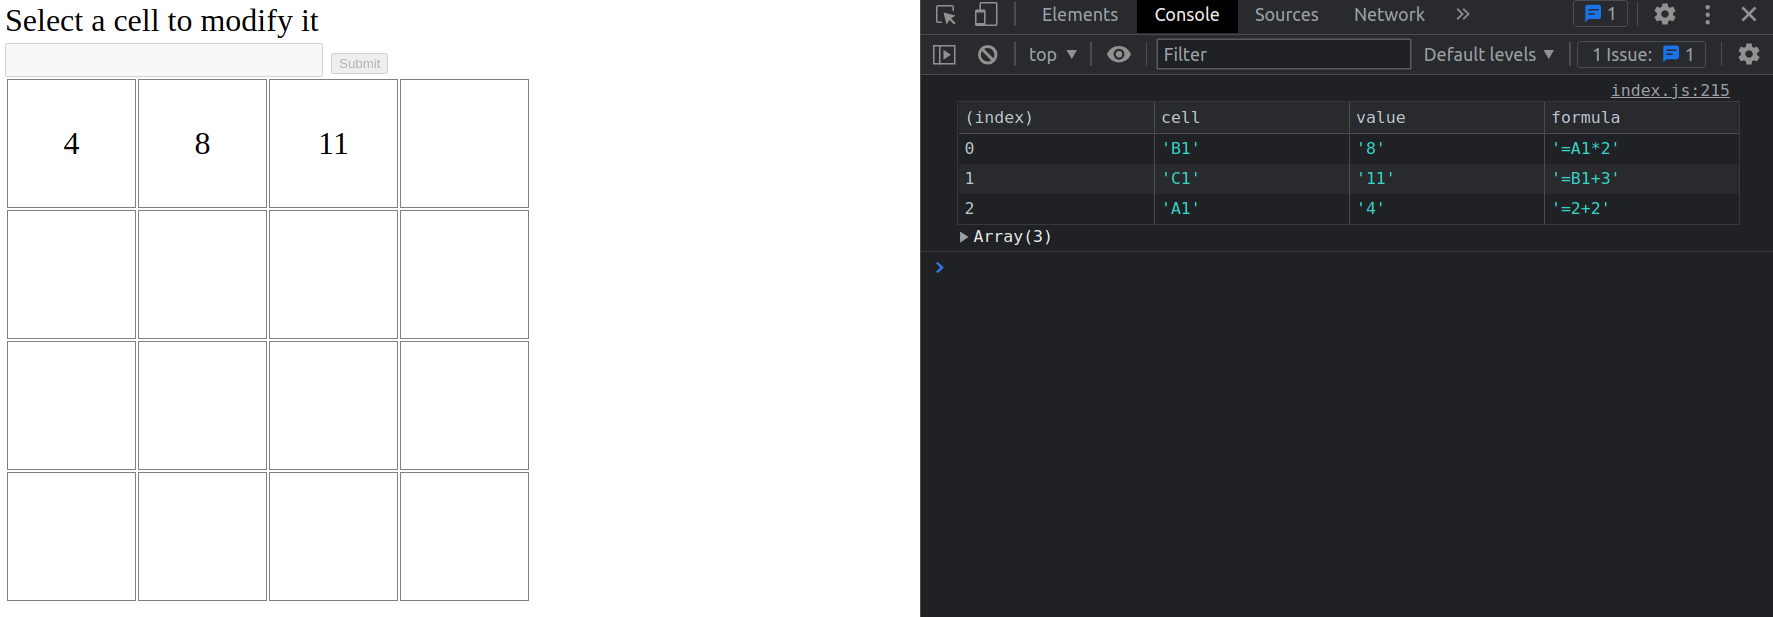
\includegraphics[width=\columnwidth]{spreadsheet-GET.png}
    \caption{When we refresh the page, or another user access, the GET methods returns the current cells}
  \end{figure}

  \pagebreak
  \section{Push system for synchronization}
  Cell modification should be shared across all connected users.

  The code between the first and the second assignment is different. In the source folder of the project it was added a zip which contains the two versions. 

  However, a prefered method of looking at the different versions is to use the git branches created: \textit{ass-1} for the first one, \textit{ass-2} for the second one (which is the same as the \textit{master} branch). By using git is it possible to simply change the branch and rebuild the server without having to manually copy the files and compile them with \textit{tsc}.

  \subsection{Front End Javascript}
  \begin{lstlisting}[language=javascript, caption={EventSource code}]
    /** inform the server of a cell modification, then use modifyCells() */
    async function serverParseFormula(formula: string) {
      if (formula.includes('"')) return alert('Invalid " character inside input');
      const server_req: Update = {
        cell: current_cell_id,
        formula,
      };

      try {
        const res_json = await fetch(url, {
          method: "POST",
          body: JSON.stringify(server_req),
        });
        const res: ServerPostRes = await res_json.json();

        if (res.success) {
          console.log("POST request was OK");
        } else {
          console.log(`POST request ERROR: ${res.reason}`);
          alert(`You made an invalid request\nReason: ${res.reason}`);
        }
      } catch (e: any) {
        console.error(e);
        alert(`Something went wrong!\nError sending changes: ${e.message}`);
      }
    }
    
    /** use EventSource to receive updates from the server */
    function receivePushNotification() {
      const source = new EventSource(url);

      source.onopen = () => {
        console.log("eventsource opened");
      };

      source.onerror = () => {
        console.log("eventsource error, reloading...");
      };

      source.onmessage = (event: MessageEvent<string>) => {
        console.log("new update received");
        const res_json = event.data;
        const res: ServerChanges = JSON.parse(res_json);
        modifyCells(res);
      };

      return source;
    }
    const source = receivePushNotification();
  \end{lstlisting}
  The only modification we need in the Javascript is that now we should not modify the cells with fetches but only with an \textit{EventSource}, which will automatically call the GET method at startup.

  We removed the \textit{getStartingValues} function and modified the POST request so that it receives only a success message. When a modification is made, the result is shared between all users and received by the \textit{EventSource onmessage} method.

  Some types names have been changed to better indicate what they do.

  \pagebreak
  \subsection{Back End Java}
  We need to keep track of the current users and their active connection. To do that, we use an HashMap of \textit{<String, AsyncContext>}. This HashMap gets updated each time a new user asks for a GET request.

  \subsubsection{GET Method}
  \begin{lstlisting}[language=java, caption={GET route, second version}]
    public void addReader(HttpServletRequest req, HttpServletResponse res) {
        // This a Tomcat specific - makes request asynchronous
        req.setAttribute("org.apache.catalina.ASYNC_SUPPORTED", true);

        final String id = UUID.randomUUID().toString();
        final AsyncContext ac = req.startAsync(req, res);
        ac.addListener(getAsyncListener(id));

        readers.put(id, ac);
        System.out.println("Added new client: " + ACToString(ac));
    } 

    @Override
    public void doGet(HttpServletRequest req, HttpServletResponse res) throws IOException {
        // System.out.println("\nNew user accessing");
        addReader(req, res);
        Set<Cell> modified_cells = engine.getUsedCells();
        sendUpdate(res, modified_cells);
    }
  \end{lstlisting}

  The GET method works mostly the same for the user. The main difference is that now the server saves the current connection for future updates.

  \pagebreak
  \subsubsection{POST Method}
  \begin{lstlisting}[language=java, caption={POST route, second version}]
    public void sendOkResponse(HttpServletResponse res) throws IOException {
        String msg = "{\"success\": true}";
        sendMessage(res, msg, "text/application-json");
    }
    
    public void sendUpdateToAllReaders(Set<Cell> modified_cells) {
        Iterator<AsyncContext> iter = readers.values().iterator();
        while (iter.hasNext()) {
            AsyncContext reader = iter.next();
            try {
                HttpServletResponse res = (HttpServletResponse) reader.getResponse();
                sendUpdate(res, modified_cells);
                System.out.println("Send message to user: " + ACToString(reader));
            } catch (Exception e) {
                System.out.println("error printing to " + ACToString(reader));
                iter.remove();
            }
        }
    }
    
    @Override
    public void doPost(HttpServletRequest req, HttpServletResponse res) throws IOException {
        //Same code to parse the JSON

        sendOkResponse(res);
        sendUpdateToAllReaders(modified_cells);
    }
  \end{lstlisting}
  
  In the second version, the updates are not send directly. Instead, we simply respond to the user making the change with a success status, and then send the update to all users (including the one who modified it).

  \subsection{Results}
  \begin{figure}[H]
    \centering
    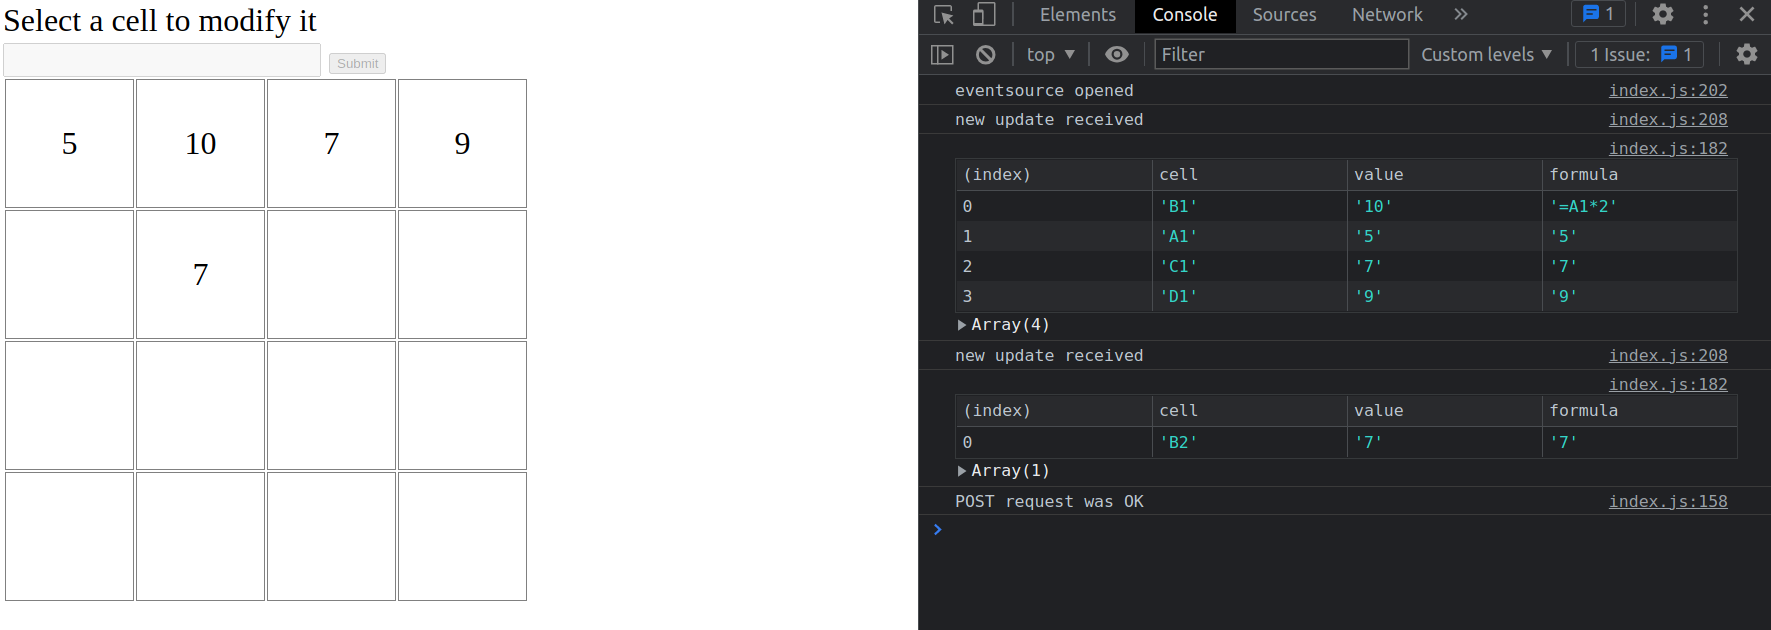
\includegraphics[width=\columnwidth]{eventsource-POST.png}
    \caption{The user receives the current state when accessing, and he is able to send an update (as seen in the log \textit{POST request was OK})}
  \end{figure}
  \begin{figure}[H]
    \centering
    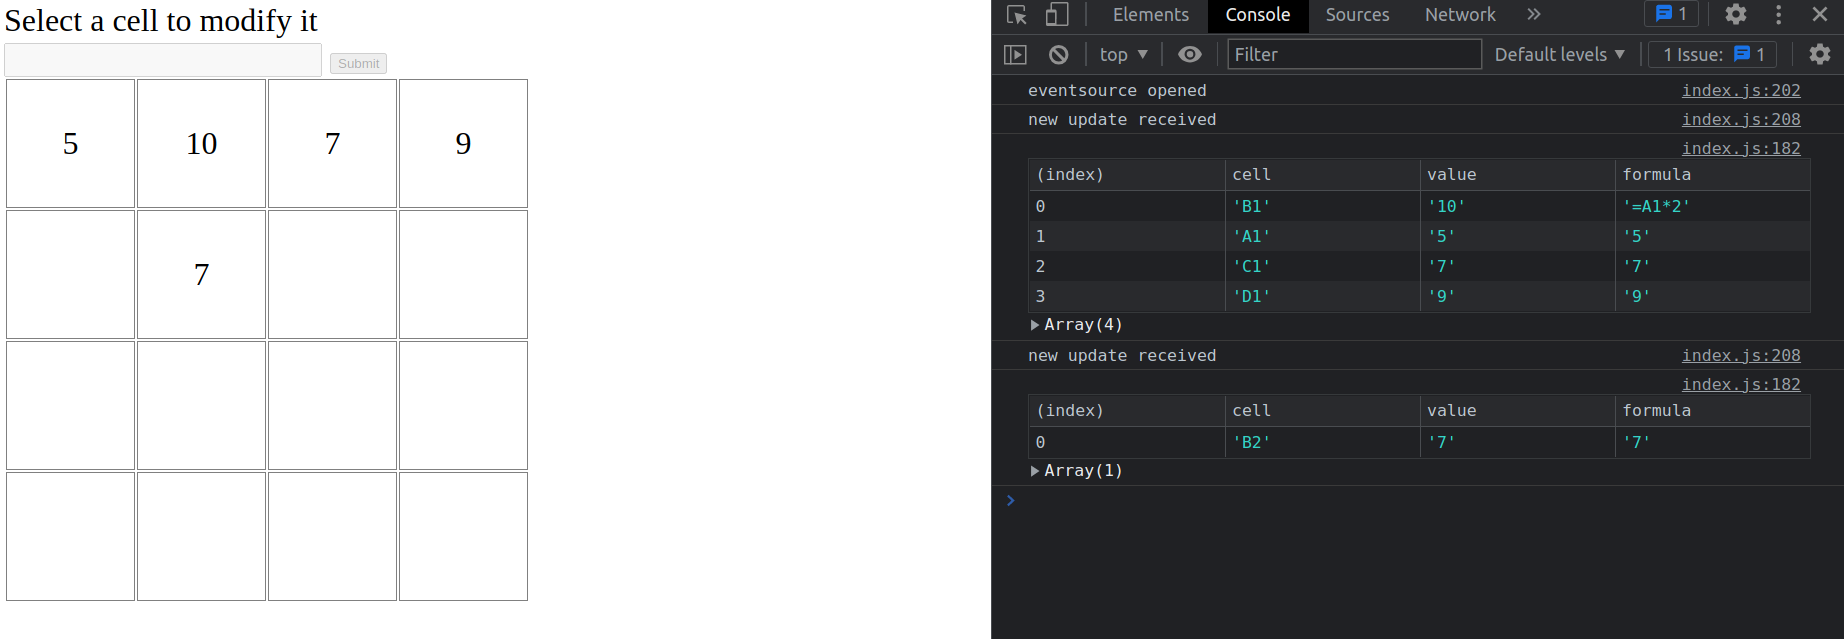
\includegraphics[width=\columnwidth]{eventsource-new-update.png}
    \caption{Other users receive the update directly without making any explicit request (the image is mostly similar, but notice the absence of the log \textit{POST request was OK})}
  \end{figure}

  \subsection{Problems}
  \begin{figure}[H]
    \centering
    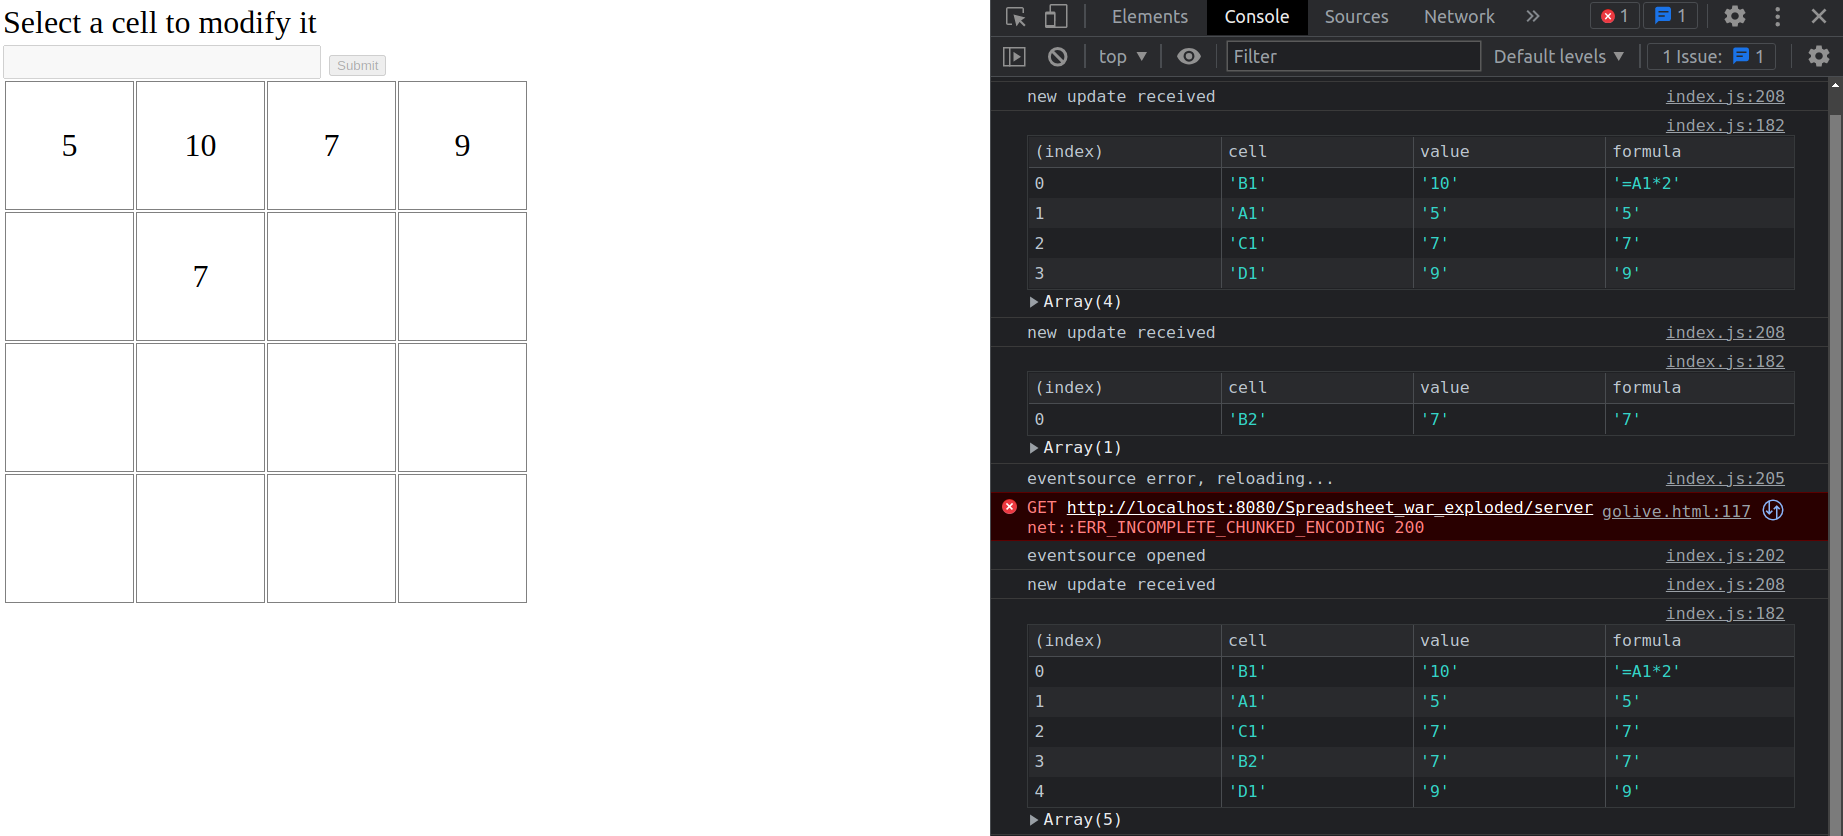
\includegraphics[width=\columnwidth]{eventsource-chrome-error.png}
    \caption{Web Browser Error}
  \end{figure}
  For unknown reasons, every thirty seconds circa the eventsource crashed giving an error code. The cause is not clear, since it may vary greatly (some users report getting it with the antivirus [https://stackoverflow.com/questions\\/29894154/chrome-neterr-incomplete-chunked-encoding-error], but it is nonsense in a linux enviroment). The error is similar in a Firefox browser.

  Solutions were tried, like sending OK message every X seconds to keep alive the connection, without success. Fortunately, if an EventSource crashed the web browser connects again: this means that the client connects like a new one every half a minute, which is inefficient, but the user should not notice such problem.

  \begin{lstlisting}[language=java, caption={example of class used to send keep alive messages, which works but does not solve the problem}]
    private class KeepAliveUsers implements Runnable {
        public void sendKeepAlive(HttpServletResponse res) throws IOException {
            String msg = "{\"success\": true}";

            res.setContentType("text/event-stream");
            res.setHeader("Access-Control-Allow-Origin", "*");
            res.setHeader("Connection", "Keep-Alive");
            res.setHeader("Cache-Control", "no-cache");
            res.setCharacterEncoding("UTF-8");
            // res.getWriter().write("event: keep-alive");
            res.getWriter().write("data: " + msg + "\n\n");
            res.getWriter().flush();
        }

        @Override
        public void run(){
            TimerTask task = new TimerTask() {
                @Override
                public void run() {
                    System.out.println("sending keep-alives...");
                    Iterator<AsyncContext> iter = readers.values().iterator();
                    while (iter.hasNext()) {
                        AsyncContext reader = iter.next();
                        try {
                            HttpServletResponse res = (HttpServletResponse) reader.getResponse();
                            sendKeepAlive(res);
                            System.out.println("Send keep-alive to user: " + ACToString(reader));
                        } catch (Exception e) {
                            System.out.println("error printing to " + ACToString(reader));
                            iter.remove();
                        }
                    }
                }
            };
            Timer timer = new Timer();
            timer.schedule(task, 0l, 1*1000l);
        }
    } 
  \end{lstlisting}

\end{document}
